\newcommand{\datawidth}{1}
\newcommand{\dataheight}{0.9}
\newcommand{\dataspacing}{0.1}

\usetikzlibrary{decorations.pathreplacing}
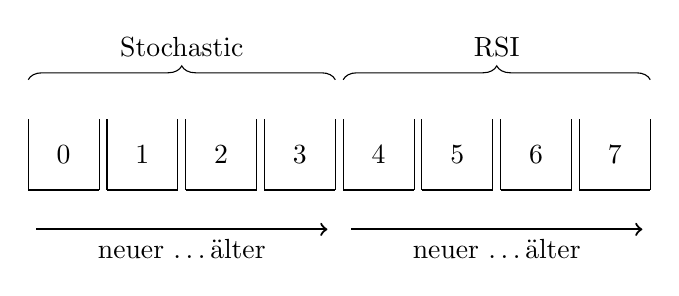
\begin{tikzpicture}
	\draw[decorate, decoration={brace, amplitude=5pt}]  (\dataspacing, 0.5) -- (4 * \datawidth, 0.5) node[midway, anchor=south, yshift=5] {Stochastic};
	\draw[decorate, decoration={brace, amplitude=5pt}]  (\dataspacing + 4 * \datawidth,0.5) -- (8 * \datawidth, 0.5) node[midway, anchor=south, yshift=5] {RSI};

	\foreach \i in {0,...,7}
	{
	        \draw (\i * \datawidth + \dataspacing, 0) -- (\i * \datawidth + \dataspacing, -\dataheight);
	        \draw (\i * \datawidth + \dataspacing, -\dataheight) -- (\i * \datawidth + \datawidth, -\dataheight);
	        \draw (\i * \datawidth + \datawidth, -\dataheight) -- (\i * \datawidth + \datawidth, 0);
	        \node[align=center] at (\i * \datawidth + 0.5 * \datawidth + 0.5 * \dataspacing, -0.5 * \dataheight) {$\i$};
	}
	
	\draw[->, thick] (2 * \dataspacing, -\dataheight - 0.5) -- (-1 * \dataspacing + 4 * \datawidth, -\dataheight - 0.5) node[midway, anchor=north] {neuer \dots älter};
	\draw[->, thick] (2 * \dataspacing + 4 * \datawidth, -\dataheight - 0.5) -- (-1 * \dataspacing + 8 * \datawidth, -\dataheight - 0.5) node[midway, anchor=north] {neuer \dots älter};
\end{tikzpicture}